\documentclass[a4paper,10pt]{article}
%\documentclass[dutch]{IEEEtran}
%\documentclass[a4paper,10pt]{scrartcl}
\usepackage{pdfpages} 
%\usepackage[dutch]{babel}
\usepackage[english]{babel}
\usepackage[utf8]{inputenc}
\usepackage[official]{eurosym}
\usepackage{listings}
\usepackage[titles]{tocloft}
\usepackage{amssymb,amsmath}
%\usepackage{caption}
\usepackage{url}
\usepackage[nottoc, numbib]{tocbibind}
\usepackage{gensymb}
\usepackage{placeins}
\usepackage{float}
%\usepackage[style=ieee, backend=bibtex]{biblatex}
 
\title{Quantified Bike}
\author{Lies Bollens \and Jakob Festraets \and Rugen Heidbuchel \and Floris Kint \and Peter Lacko}
\date{\today}

\pdfinfo{%
  /Title    (Quantified Bike)
  /Author   (Team CWA3: Lies Bollens, Ruben De Clercq, Jakob Festraets, Rugen Heidbuchel, Floris Kint, Peter Lacko)
  /Creator  ()
  /Producer ()
  /Subject  ()
  /Keywords ()
}
\setlength{\footskip}{100pt}
\begin{document}
%\maketitle
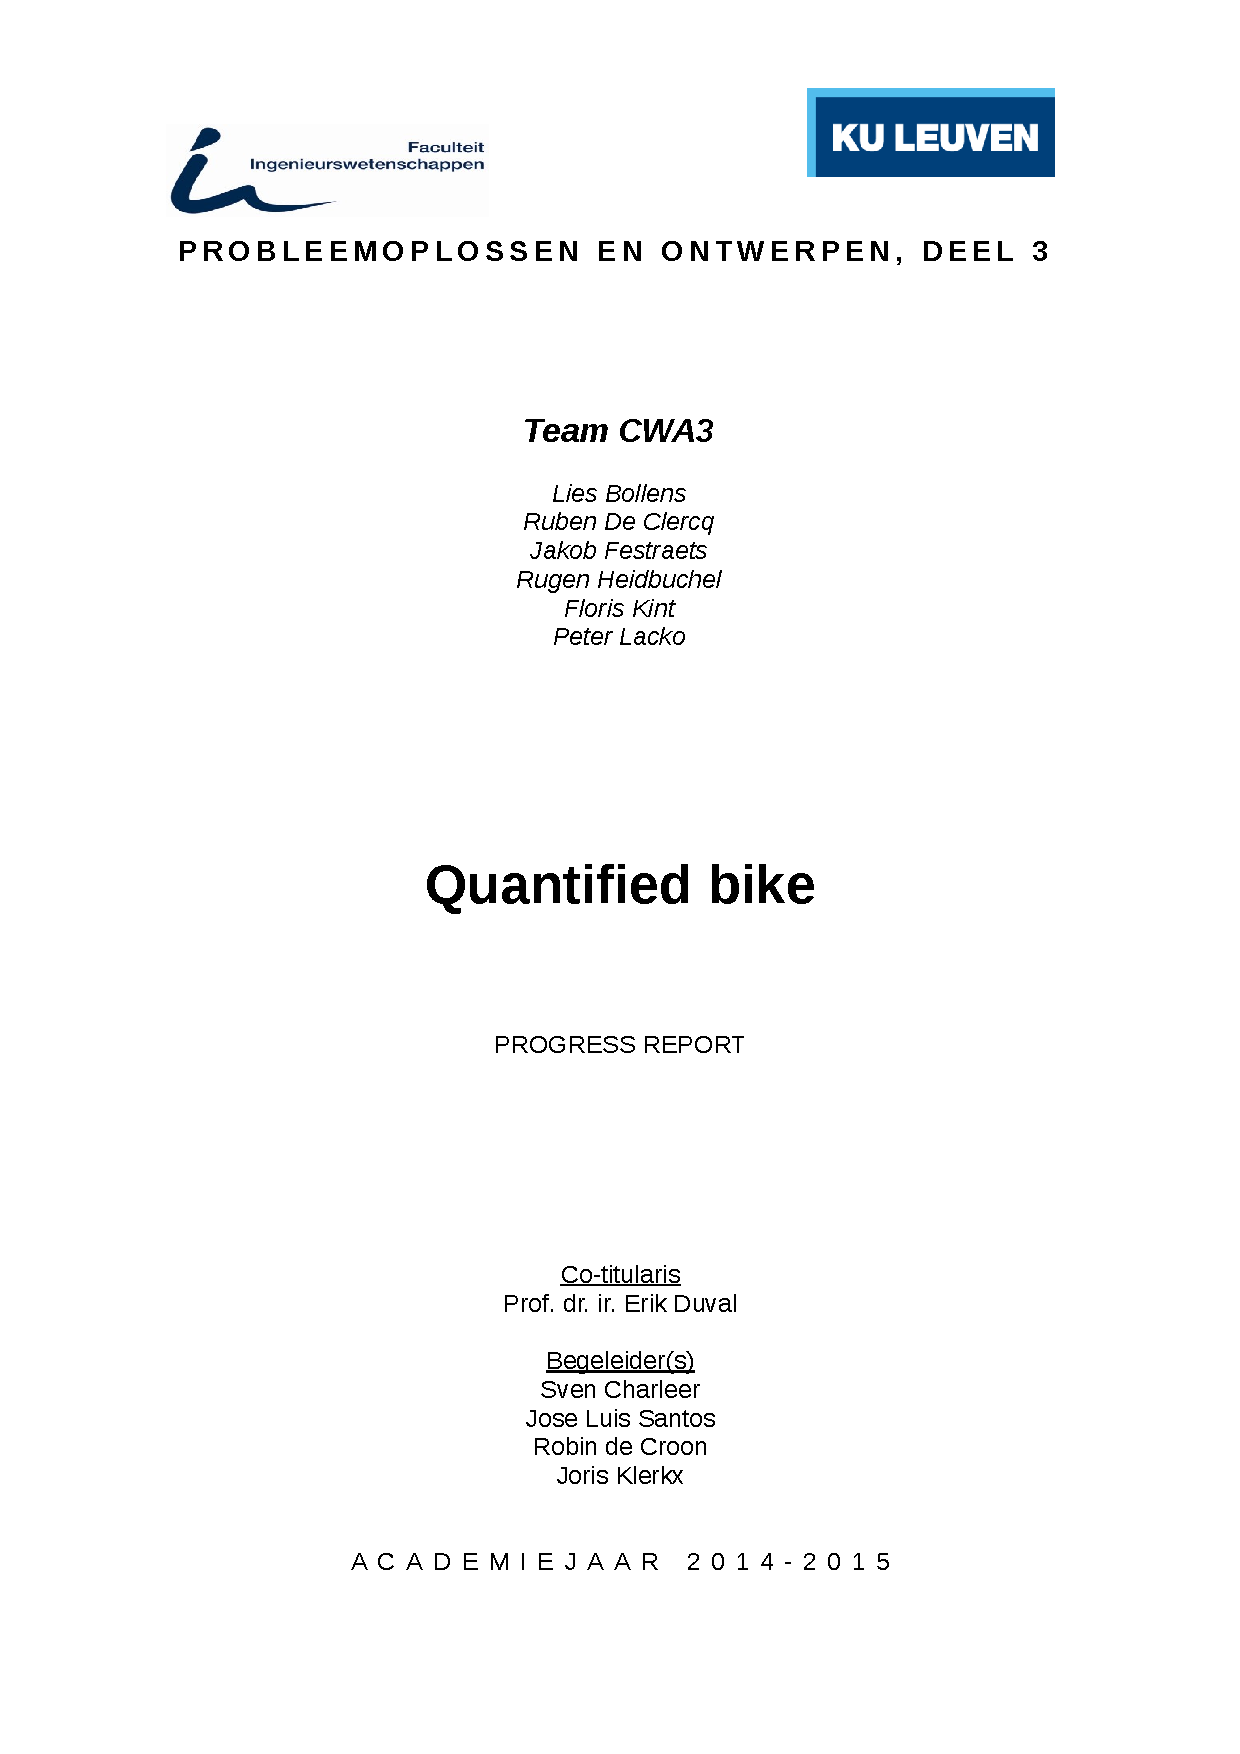
\includepdf[pages={-},pagecommand={}]{voorbladtv1415.pdf}
\newpage
\tableofcontents
\newpage
\listoffigures
%\newpage
%\listoftables
\newpage
%\section{Appendix: Workload}
\begin{figure}[H]
  \center
  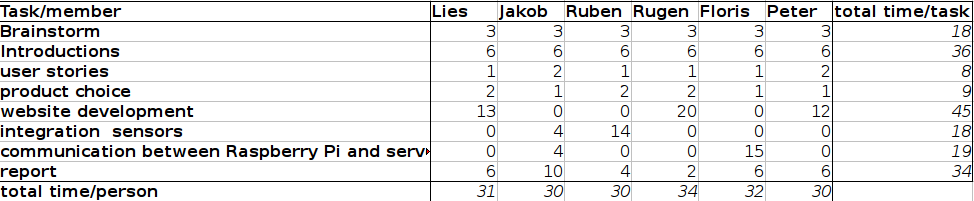
\includegraphics[width=1.5\linewidth, angle=90]{./appendix_working_times/workload.png}
  \caption{Working Times}
  \label{image:workload}
\end{figure}

\section{Group members}
The group consists of the following members.
\begin{enumerate}
 \item Lies BOLLENS, Bachelor of Science in de ingenieurswetenschappen, 2nd year
 \item Ruben DE CLERCQ, Bachelor of Science in de ingenieurswetenschappen, 2nd year
 \item Jakob FESTRAETS, Bachelor of Science in de ingenieurswetenschappen, 2nd year
 \item Rugen HEIDBUCHEL, Bachelor of Science in de ingenieurswetenschappen, 2nd year
 \item Floris KINT, Bachelor of Science in de ingenieurswetenschappen, 2nd year
 \item Peter LACKO, Bachelor of Science in de ingenieurswetenschappen, 2nd year
\end{enumerate}

\section{Brainstorm}

\begin{figure}[H]
\center
 \includegraphics[width=\linewidth]{brainstorm/brainstorm1.jpg}
 \caption{First brainstorm}
 \label{image:ganttchart}
\end{figure}
\begin{figure}[H]
\center
 \includegraphics[width=\linewidth]{brainstorm/brainstorm2.jpg}
 \caption{Second brainstorm}
 \label{image:ganttchart}
\end{figure}
A list of all the ideas created during the brainstorm.
\begin{enumerate}
 \item Using a smartphone
 \begin{enumerate}
 \item get real-time feedback
 \item play music/ put on a light
 \item take pictures of yourself/ your surroundings 
 \item easily find where your bike is parked
 \item view in an instance where your friends are
 \end{enumerate}
 \item using a GPS
  \begin{enumerate}
  \item get the fastest way from one point to another
  \item display a card, showing all the places you have been to with your bike. 
  \item Make an altitude map
  \item Easily track the distances you've covered.
  \item display some points of interest ( ex. All the pizza restaurants nearby)
  \end{enumerate}
  \item try to make your trip as efficient as possible
  \begin{enumerate}
  \item avoid red lights, based on your previous bike trips
  \item get a map, displaying the quality of the roads 
  \item find out during which moment of the day you cover a certain way the fastest
  \item get the average time needed to brake
  \item view your speed, based on the altitude difference, the temperature, the hour,...
  \item avoid bad ways 
  \end{enumerate}
  \item monitor your health
  \begin{enumerate}
   \item how many calories have you lost
    \item how much water do you need 
  \end{enumerate}
\end{enumerate}


The initial idea was to use a smartphone, since these devices contain almost all the sensors needed for the project. 
This way, creating an app for Android and iPhone devices would be enough for the concept to be functional. 
The assignment, however, was to incorporate an Arduino Nano and a Raspberry Pi. 
Since using a smartphone, an Arduino and a Raspberry Pi would get a bit too complicated, our team decided against using a smartphone. 
This meant that there would not be any screen attached to the Boss device anymore. 
Real-time communication with the user was therefore no longer possible and functions such as find-your-friends and find-your-bike not doable anymore. 

A lot of the ideas created during the brainstorm, focused on getting an augmented bike. 
This is not what the Boss device was aiming for: the purpose of this project was to create an quantified bike device, without looking at the augmented side of a bike trip. 
Once this goal had been set, a lot of the brainstorm ideas could be thrown overboard: get the fastest way, view your calorie deficit, see how much water you need, locate your friends, get points of interest,...

The idea of trying to avoid red lights seemed very appealing at first, but turned out to be too difficult to implement. 
It would require an accurate route planner that constantly refreshed, while taking all the red lights in the area into account. 
A second reason against this idea was the fact that, as a lot of other ideas, it is much more on the augmented than on the quantified side of a bike trip. 
\section{Product}
\subsection{User stories}
\subsubsection{Comparing daily trips}
Sophia uses her bike and the BOSS on a daily basis. 
She bikes to class every day and clips the BOSS on and off her bike so it does not get stolen. 
On the BOSS website, she can easily review each trip she made in the calendar overview. 
She can get a general impression of how she did each day, and then she can compare her stats with a ranked list of the stats of her friends. 
This includes the farthest traveled distance, the longest bike trips (in time), the fastest speeds, etc.

\subsubsection{Sharing biking experiences with friends}
Luke likes to go on bike trips for fun and exercise. 
He sometimes doesn’t know where he will go, but he can easily find out where he’s been in the BOSS’s detail page on the website. 
When he sees a beautiful view, or just something interesting, he can easily take a picture on the built-in camera with a click of a button. 
He can also press a second button to mark certain points of interest. 
The points of interest are displayed with the photos on a map of his route that he can share with his friends on various social media sites (Facebook, Twitter, Google Plus,…) On top of the map, he can share various statistics of his trip (how bumpy the road was, how fast he went, how hot and humid it was) along with personal comments and ratings. 
If he wants, he can also view the statistics and comments of fellow cycling friends. 

\subsubsection{Fitness stats}
Johnny likes biking for sport, and loves using the BOSS to record his data. 
He always keeps the BOSS on his bike, and only has to flick a switch to turn it on or off. 
After each ride, he goes to the BOSS website to check specific details of how he did, and can compare his performance with previous rides, made possible by the detailed compare view of the BOSS website. 
Furthermore, he can also compare his data with his competitive friends, by use of simple numbers (for the mean speed, travel distance and travel time), or with graphs (speed during a trip, measured temperature throughout the trip, heart rate, etc.) Finally, he can challenge his friends to beat his results via various social media sites.

\subsection{Product description}
The BOSS records several different types of data with external sensors that are either connected to the Raspberry Pi or the Arduino Nano. 
If an internet server is available, the data is sent to the server. If the connection is lost, the data can be stored locally.
It also has three input buttons: there is a switch to turn it on or off, a button to take a picture with a camera and a button to indicate a point of interest. 
The data from the last two are combined with recorded GPS data. Exterior LEDs indicate whether the connection to the server is working or not.
The website starts with the user’s own dashboard, showing random statistics of them and their friends. 
Here they can either choose to go to their personal (calendar) view, or compare and share with their friends in the social view. 
The calendar view gives the user an overview of their rides on each day, and a more detailed view per day after the user requests it. 
They can also compare multiple days by selecting the chosen days in the calendar view. 
The social view allows the user to compare his statistics with a friend, or find multiple rankings based on different statistics (e.g. highest speed, most distance traveled, longest bike ride).
The user can also share his results and challenge friends on multiple social media sites.

\section{Brainstorm}

\section{Used technologies}
\subsection{Device}
\subsubsection{Python}
Libraries
\begin{enumerate}
 \item python-serial
 \item SocketIO
\end{enumerate}
\paragraph{Threads}
The application on the Raspberry Pi uses threads so the application can simultaneously read data from the Serial Interface to the Arduino and send data to the local database or the server.
\subsubsection{MySQL}
When the application can't send data to the remote server, all data is stored on a local MySQL database. MySQL is an open source relational database engine.
\subsubsection{Web sockets}
\subsubsection{Raspberry Pi}
\subsubsection{Arduino Nano}
The Arduino Nano is a single-board microcontroller, which can be used to simplify building an interactive environment. It gives us the advantage that it becomes rather easy to connect and read sensors and the like, which else would have been a difficult job. A disadvantage to the Arduino however, is the fact that it can only run one thread at a time. This makes reading multiple sensors slightly harder. For example, the GPS module has to wait for a signal, while the temperature sensor gives us a constant signal. Luckily, it still is possible to program the Arduino so that it can read all sensors on the right time and process all the data to the Raspberry Pi.
To make it possible for the Arduino to read the sensors, we use some custom-made libraries.
\begin{enumerate}
 \item DHT11 for the temperature-humiditysensor
 \item Adafruit_GPS for the GPS module
\end{enumerate}

\subsection{Web interface}
\subsubsection{Javascript}
Javascript is a programing language used to program the behavior of a web page. It is easy to implement in a HTML file. An advantage of Javascript is that it is executed on the client side. This way, the web server won't unnecessarily be strained. A disadvantage is that a lot of lines have to be written in order to get some basic functionality. 
In this project, Javascript is used to create all the functionality on the client site. Without Javascript, the client site would not be able to get any data from the server and would thus be useless. 

\subsubsection{JQuery}
Jquery is a JavaScript library, created to simplify JavaScript programming. Using JQuery, lots of commands are simplified. In almost every JavaScript document used in this project, JQuery commands are present. 
For the calendar, an external Jquery library 'DataTables' was used. 
\textbf{RUGEN schrijf hier nog bij}

\subsubsection{JSON}
JSON is a data interchange format. Although it stands for JavaScript Object Notation, it is language independent. JSON is relatively easy to understand and is faster than other similar formats. In this project, JSON is used for data interchange between the client site and the data bank. 

\section{Course Integration}
This project focuses on Informatics, but of course Mathematics is always present.
\subsection{Informatics}
We make use of Informatics to design the architecture of our application and to write our
software. This course has helped us to design our data models and to think about how
functionality should be divided into logical parts (classes).
\subsection{Mathematics}
\subsubsection{Statistics}
To analyse our measured data we make use of Statistics. This also helps to take
measuring errors into account.
\subsubsection{Numerical Mathematics}
All measured values are liable to measuring errors. These errors influence all further
calculations. Luckily our data does not need to be super exact. Our GPS data for example
only has to be closely to a few meters.
\section{Conclusion}
<<<<<<< HEAD
We already learned a lot in this project. First of all, we learned how to combine an
Arduino with a Raspberry Pi. Secondly, we learned a lot about web technologies. We now
know how to write webpages using the combination of HTML, CSS and javascript (with
jQuery). Thirdly, we learned how to use the version management system called git.

We think the introduction sessions where good. They weren't too long and gave a short summary of what every technology was meant for.Those who didn't know these
technologies yet, could go through some tutorials. The only thing we did not like about the project, was the focus on 
a quantified bike. We would have prefered a combination of a quantified and an augmented bike, since an augmented bike
has a lot more applications in real-life. It would be easier to imagine a user public and to implement a useful application.

We still plan to make use of SCSS, to easily change global parameters like our base colour.

\section{Appendix: Workload}
\begin{figure}[H]
  \center
  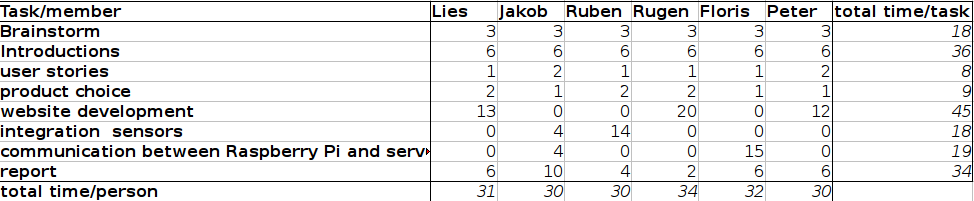
\includegraphics[width=1.5\linewidth, angle=90]{./appendix_working_times/workload.png}
  \caption{Working Times}
  \label{image:workload}
\end{figure}

\section{Appendix: Planning}
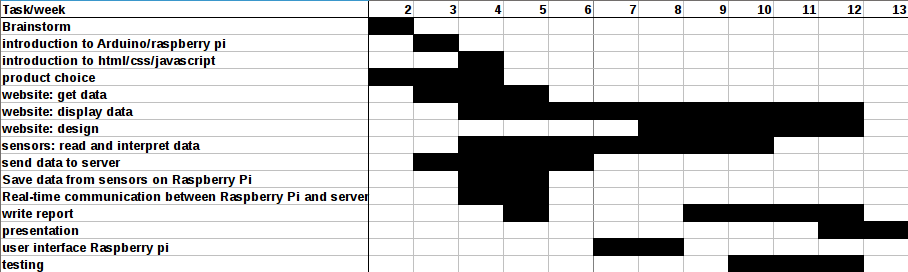
\includegraphics[width=5in]{./appendix_planning/ganttchart.png}
\section{Attachments}
\subsection{Brainstorm pictures}
\label{subsection:brainstorm-pictures}
\begin{figure}[H]
\center
 \includegraphics[width=\linewidth]{attachments/brainstorm/brainstorm1.jpg}
 \caption{First brainstorm}
 \label{image:ganttchart1}
\end{figure}
\begin{figure}[H]
\center
 \includegraphics[width=\linewidth]{attachments/brainstorm/brainstorm2.jpg}
 \caption{Second brainstorm}
 \label{image:ganttchart2}
\end{figure} 

\subsection{Screenshots}
\label{subsection:screenshots}
\begin{figure}[H]
\center
 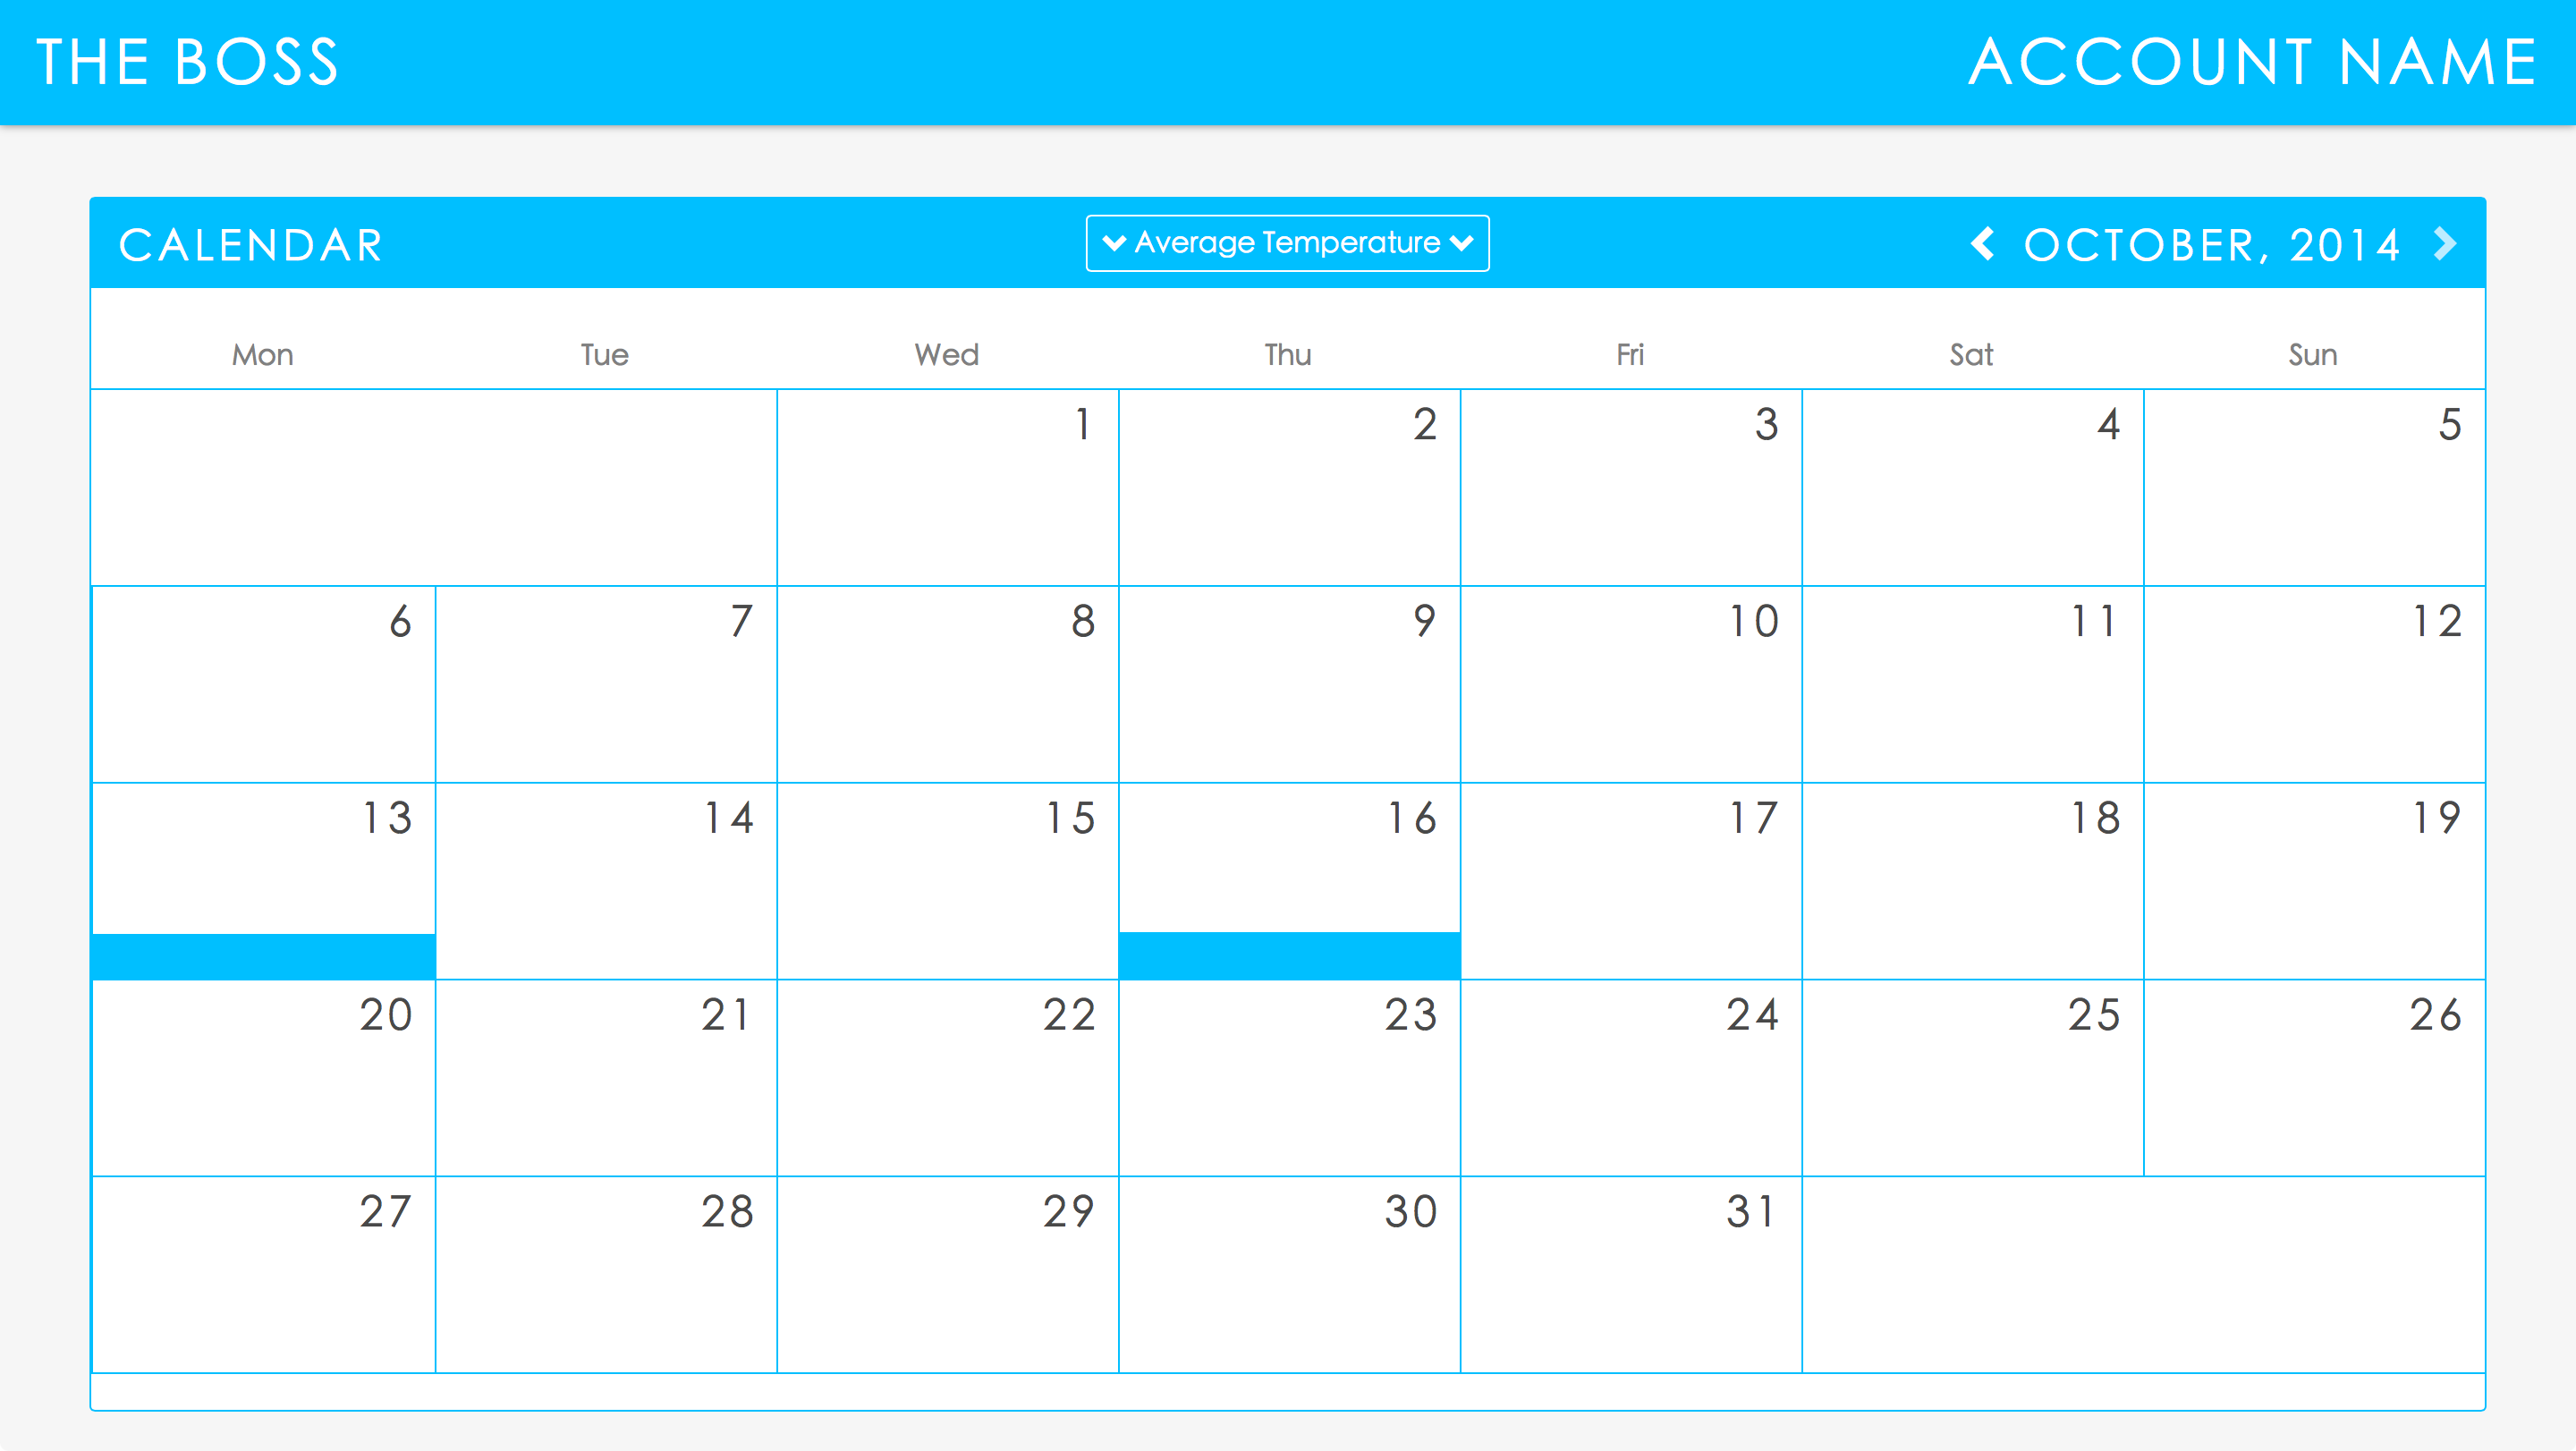
\includegraphics[width=\linewidth]{attachments/screenshots/CalendarView.tiff}
 \caption{Main calendar view}
 \label{image:screenshot1}
\end{figure}
\begin{figure}[H]
\center
 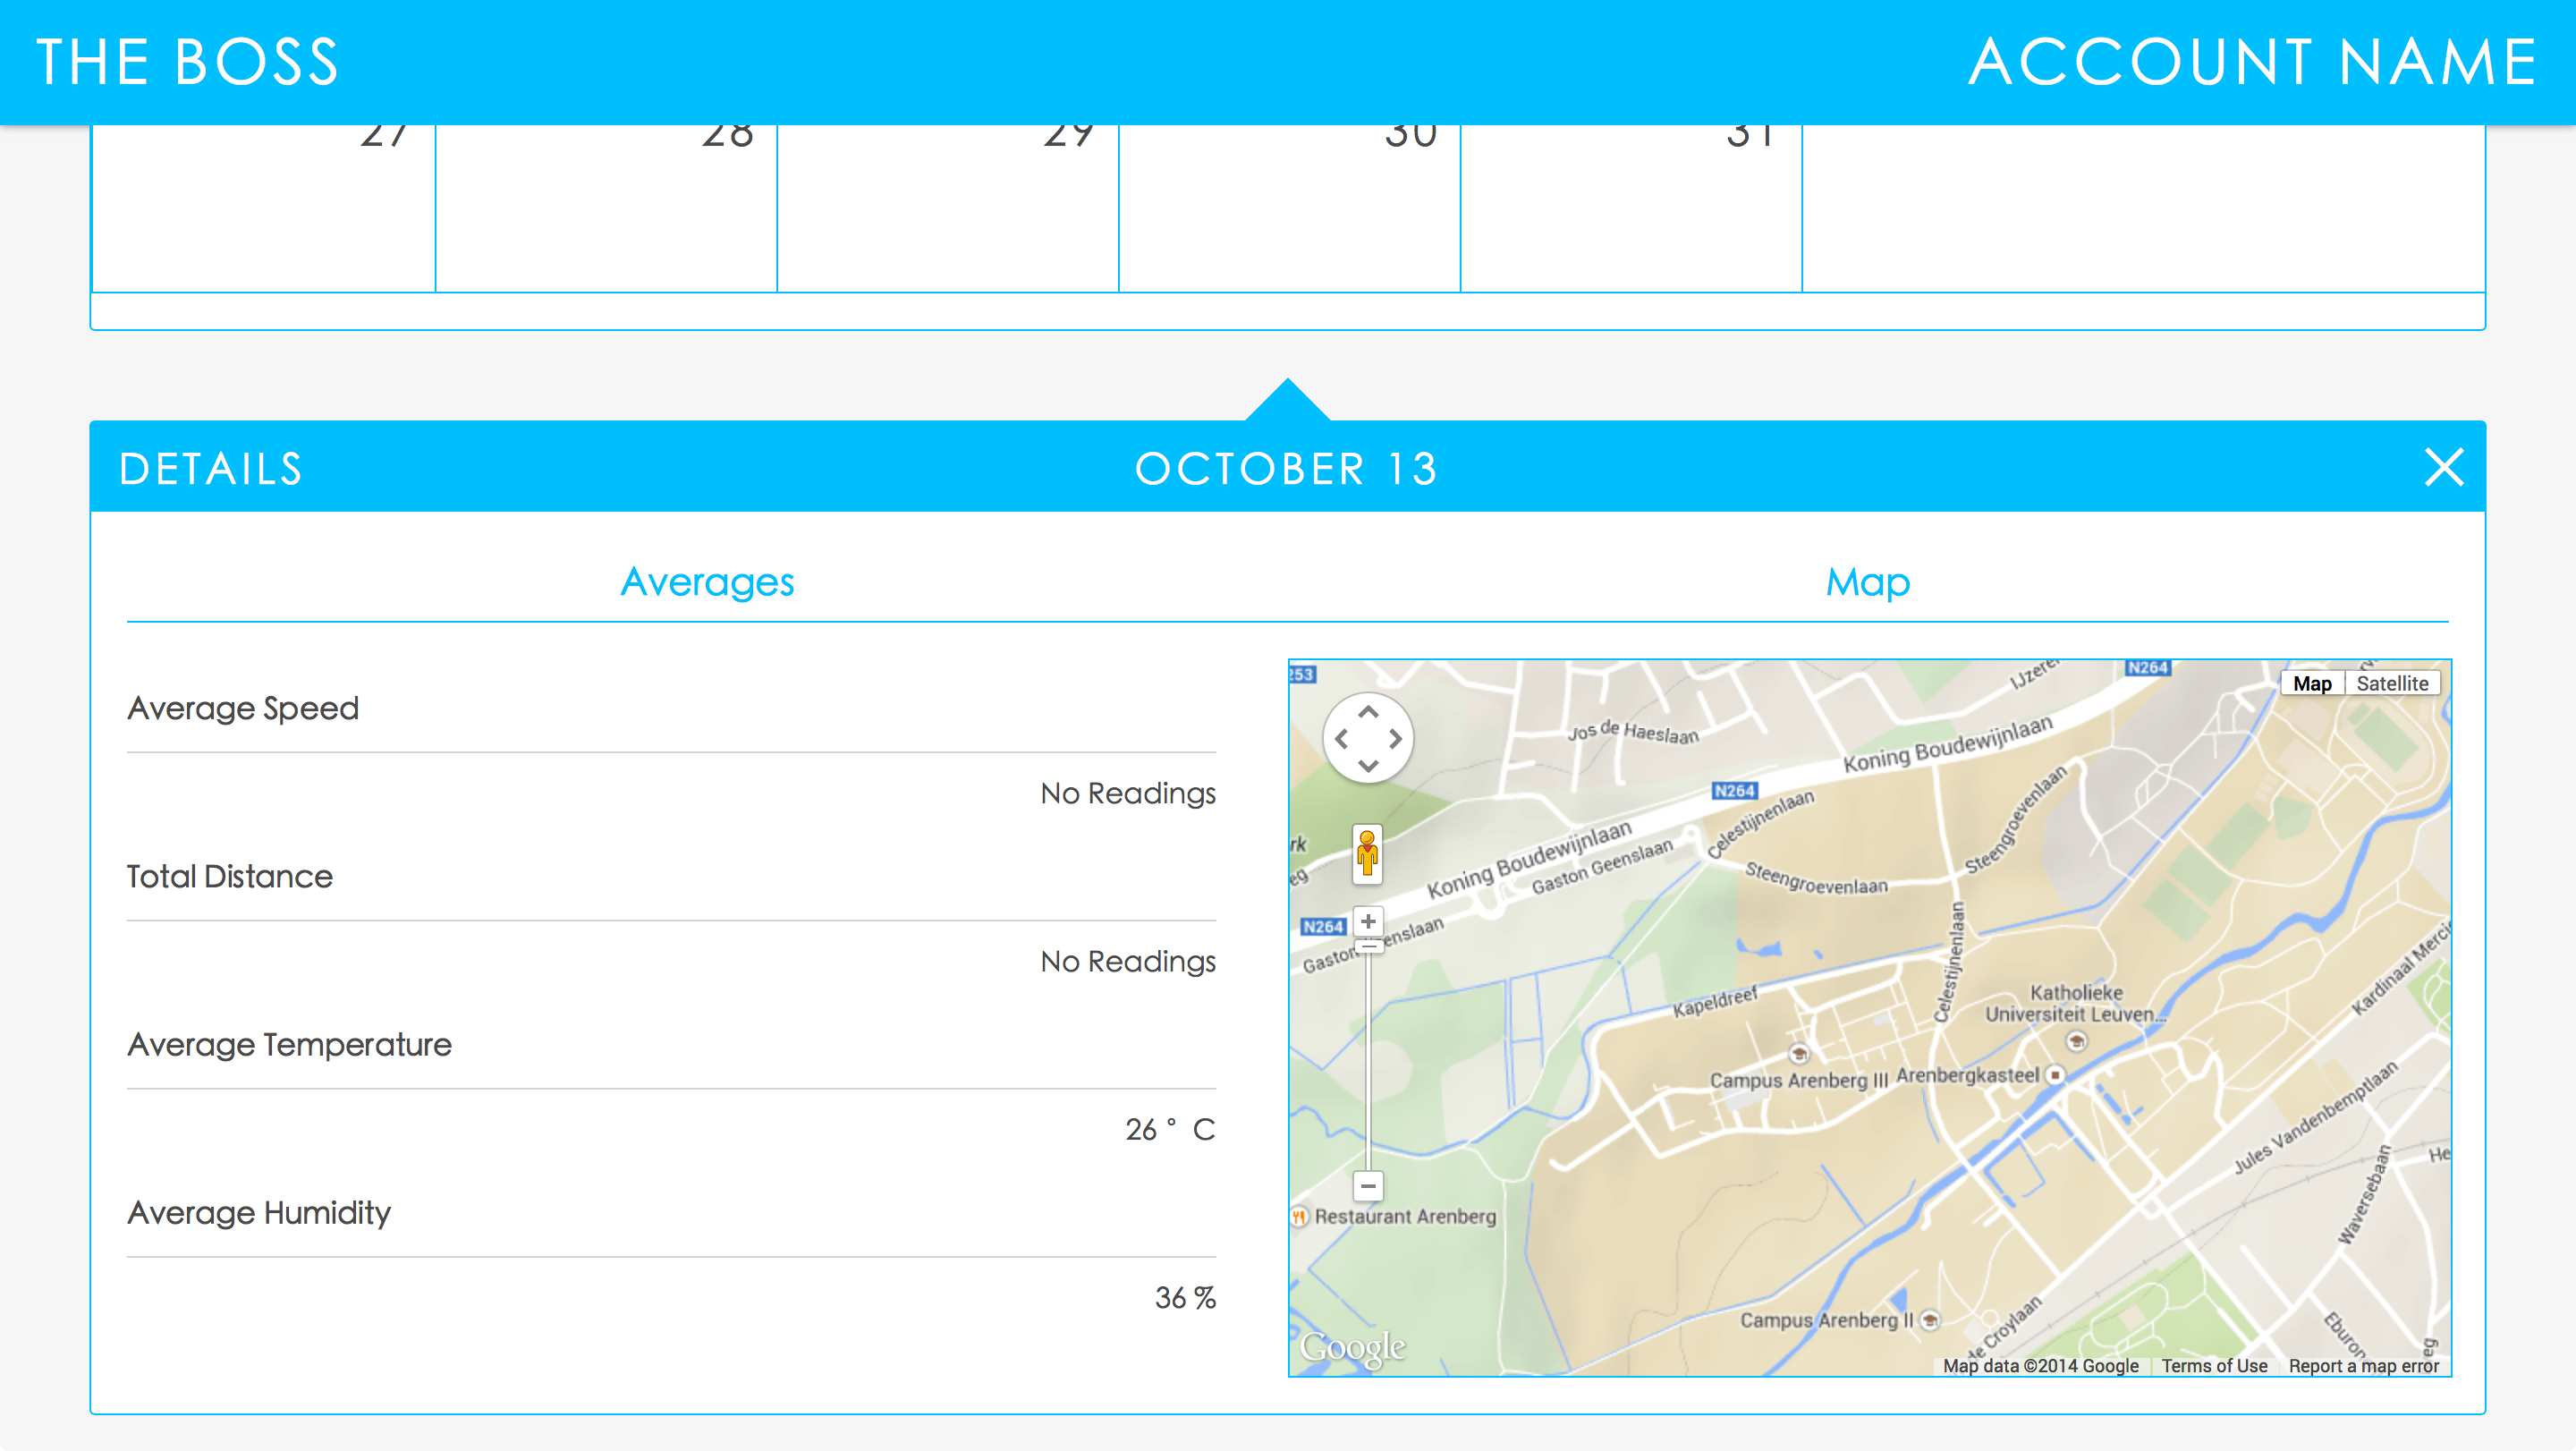
\includegraphics[width=\linewidth]{attachments/screenshots/DetailsSection.tiff}
 \caption{Details section}
 \label{image:screenshot2}
\end{figure} 


\bibliographystyle{IEEEtran}
\bibliography{referenties}{}

\end{document}
